% !TEX program = xelatex
\documentclass[tikz, crop, border = {2pt 2pt 2pt 2pt}]{standalone}

\usetikzlibrary{decorations.pathreplacing, calligraphy}
\usetikzlibrary{calc}

\usepackage{concmath-otf}

\begin{document}
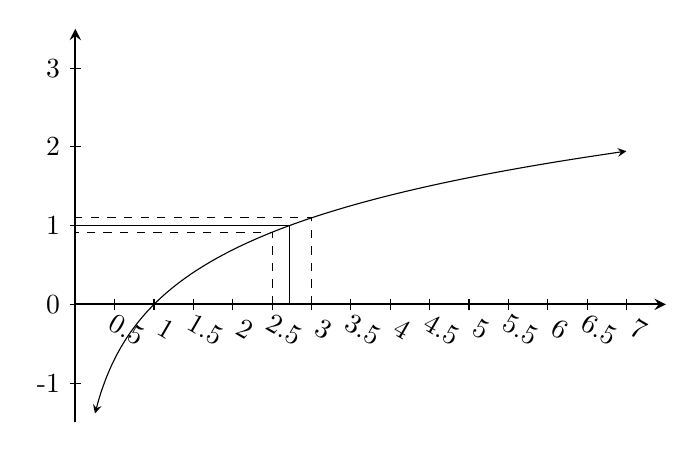
\begin{tikzpicture}
	\draw[thick, -stealth] (0, 0) -- (7.5, 0);
	\draw[thick, -stealth] (0, -1.5) -- (0, 3.5);

	\foreach \x in {0.5, 1, ..., 7} {
			\draw (\x, 2pt) -- ++ (0, -4pt) node[yshift = -0.25cm, xshift = 0.15cm, rotate = -30]{$\x$};
		}
	\foreach \x in {-1, 0, ..., 3} {
			\draw (2pt, \x) -- ++ (-4pt, 0) node[left]{\x};
		}
	\draw[smooth, domain = 0.25:7, stealth-stealth] plot[samples=100] (\x, {ln(\x)});

	\draw (2.717, 0) |- (0, 1);
	\draw[dashed] (2.5, 0) |- (0, 0.916);
	\draw[dashed] (3, 0) |- (0, 1.098);
\end{tikzpicture}
\end{document}
